
\cxset{style19/.style={
 name={},
 numbering=arabic,
 number font-size=Huge,
 number font-family=rmfamily,
 number font-weight=bfseries,
 number before=\par\offinterlineskip,
 number after=\kern0.5em,
 number dot={ },
 number position=rightname,
 chapter font-family=rmfamily,
 chapter font-weight=mdseries,
 chapter font-size=Huge,
 chapter before=\par,
 chapter after=\par,
 chapter color=black!90,
 number  color=black!90,
 chapter title width=0.8\textwidth,
 chapter title align=left,
 title   beforeskip=,
% title afterskip={\vspace*{50pt}\par},
 title margin top=0pt,
 title margin bottom=50pt,
 title margin-left=0pt,
 title before=,
 title after=\par,
 chapter title text-align=left,
 title font-family=rmfamily,
 title font-color=black!90,
 title font-weight=bfseries,
 title font-size=Huge}}
 
\parindent1em

\cxset{style19}
\chapter{Introduction to chapter style nineteen}

I first visited the Gulf seven years after its independence. As Simon C. Smith puts it, in his book \emph{Britain’s Revival and Fall in the Gulf} the decolonization of the Gulf was a mere footnote on British history. As I have lived in and I am currently still working in the area in this footnote for about twelve years Smith’s book sheds light to the beginnings of the Gulf.

\medskip
\begin{figure}[ht]
\centering 
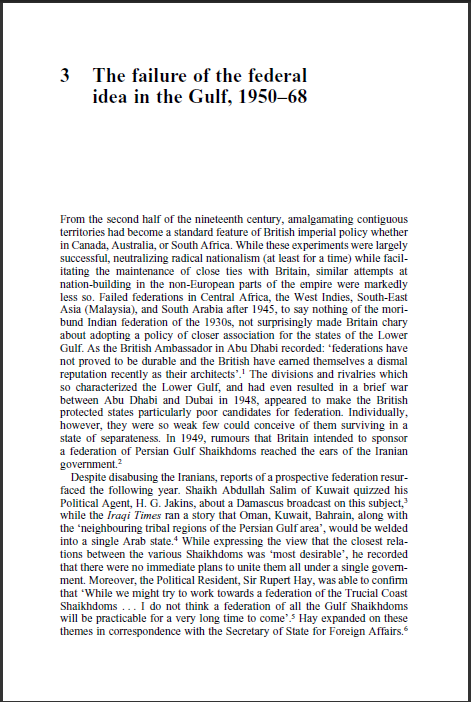
\includegraphics[width=0.5\textwidth]{./chapters/chapter19.png}
\end{figure}

The book’s typography is what one expects from an academic publication. The headings are simple and the text is typeset in Times Roman. I was tempted to name this template \emph{plain vanilla} but perhaps it deserves better.
There is a large section of book designers that believe that the typography of a book should be like a crystal glass.

\begin{quote}
Now the man who first chose glass instead of clay or metal to hold his wine was a ``modernist" in the sense in which I am going to use that term. That is, the first he asked of this particular object was not "How should it look?" but ``What must it do?" and to that extent all good typography is modernist.	
\end{quote}

Throughout the essay, Warde argues for the discipline and humility required to create quietly set, ``transparent" book pages.

Now, back to the template one of the difficulties we will face is that the chapter title blocks are set in Once we adjust the title to be anything less than the width of the text block, we will also need to be careful
about words in order to give it some balance.
two or three lines and they do not extend to the full length of the text block.

The main settings are as follows:

\begin{verbatim}
\cxset{reset,
 chapter title width=0.65\textwidth,
 chapter title align=raggedright,}
\end{verbatim}


\cxset{chapter opening=anywhere}
\chapter{The failure of the federal idea in the Gulf, 1950-68}

The book does not have any lower level headings. Another characteristic is a subtitle below the main chapter block on some of the chapters. The subtitle is set in normal weight and is \emph{partially} used as a heading. 

\testsections




